\documentclass[12pt]{article}
\usepackage[spanish]{babel}
\usepackage[utf8]{inputenc}
\usepackage{amsmath}
\usepackage{listings}
\usepackage[usenames]{color}
\definecolor{gray97}{gray}{.97}
\definecolor{gray75}{gray}{.75}
\definecolor{gray45}{gray}{.45}
\definecolor{azul1}{RGB}{141,198,163}
\definecolor{azul2}{RGB}{24,107,122}
\definecolor{verde1}{RGB}{44,186,34}
\usepackage{graphicx}
\usepackage{caption}
\usepackage{subcaption}
\usepackage{textcomp}
\lstset{
		frame=Ltb,
		framerule=1pt,
		framextopmargin=5pt, %margen de arriba
		framexbottommargin=5pt, %margen de abajo
		framexleftmargin= -2pt, %separacion del margen izquierdo
		framesep=2pt,
		rulesep=0.2pt,
		backgroundcolor=\color{gray97},
		rulesepcolor=,
        tabsize=4,
        rulecolor=\color[RGB]{106, 182, 217}, %AZUL
        upquote=true,
        aboveskip={1.5\baselineskip}, %despues de la linea de texto
        columns=fixed,
        showstringspaces=false,
        extendedchars=true,
        breaklines=true,
        prebreak = \raisebox{0ex}[0ex][0ex]{\ensuremath{\hookleftarrow}},
        showtabs=false,
        showspaces=false,
        showstringspaces=false,
        basicstyle=\scriptsize\ttfamily\color[RGB]{39, 100, 46}, %Numeros de lineas, simbolos, puntos y coma y demas
        identifierstyle=\ttfamily\color[RGB]{56, 140, 189}, %variables
        commentstyle=\color[RGB]{62, 179, 101}, %comentarios
        stringstyle=\color[RGB]{247, 165, 42}, %impresiones
        keywordstyle=\bfseries\color[RGB]{237, 118, 150}, %funciones
        %
		numbers=left,
		numbersep=-7pt, %separacion del numero
		numberstyle=\tiny,
		numberfirstline = false,
		breaklines=true,
		}
\usepackage{graphicx}
\usepackage[colorinlistoftodos]{todonotes}
\usepackage{natbib} %citas bibliograficas estilo APA :p
\usepackage{eso-pic}
\usepackage{avant}
\usepackage[top=2cm,bottom=2cm,left=2.5cm,right=3cm,headsep=8pt,a4paper]{geometry}
\usepackage{fancyhdr}
\pagestyle{fancy}
\fancyhf{}
%\fancyhead[LE,RO]{}
\fancyhead[RE,LO]{Procesamiento de Señales II}
\fancyfoot[CE,CO]{\leftmark}
\fancyfoot[LE,RO]{\thepage}
\renewcommand{\headrulewidth}{2pt}
\renewcommand{\footrulewidth}{1pt}
\usepackage{tabu}
\usepackage{array}
\usepackage{multirow}
\usepackage{amssymb}
\usepackage{makeidx}
\graphicspath{ {images/} }
\usepackage{wrapfig}
\usepackage{enumerate}
\usepackage{amsmath,tikz}
\usetikzlibrary{matrix}
\usepackage{steinmetz}
\newcommand*{\horzbar}{\rule[0.05ex]{2.5ex}{0.5pt}}
\usepackage{calc}
\date{\today}


\begin{document}

\begin{titlepage}
\newcommand{\HRule}{\rule{\linewidth}{0.5mm}} 
\center
\textsc{\LARGE  Benemérita Universidad \\[0.2cm] Autónoma de Puebla}\\[1.5cm] 

\includegraphics[width=4cm]{escudo.jpg}\\[1cm]
\textsc{\Large Facultad de Ciencias de la Electrónica}\\[0.5cm] 
\textsc{\large Licenciatura en Electrónica}\\[0.5cm]
\HRule \\[0.4cm]
{ \huge \bfseries Práctica 3}\\[0.4cm] 
\HRule \\[1.5cm]
\begin{minipage}{\textwidth}
\center 

\emph{Profesor:} \\
Fernando López Marcos \\[1cm]

\begin{tabular}{ll}
\emph{Alumnos:} & \emph{Número de Matrícula:}\\
Hanan Ronaldo Quispe Condori  & 555010653 \\
Erick Sandro Niño García & 201631150\\
Carlos Alfredo Vega Aguilar & 201632131 \\
\end{tabular}
\end{minipage}\\[2cm]
\today
\end{titlepage}

%\newpage
%~\vfill
%\thispagestyle{empty}
%\begin{figure}[hbtp]


%\includegraphics[width=4cm]{IMAGENES/motordc}
%\end{figure}
%\noindent \textsc{Trabajo Encargado: Problemas en MatLab \\ Máquinas Eléctricas \\ Universidad Nacional de San Antonio abad del Cusco}\\
%noindent \textsc{Ingeniería Electrónica }\\
%\noindent \textit{Tercera revisión, \today}

%\tableofcontents indice bloqueado xD

\newpage

\section{Introducción}
 Con el desarrollo de ésta práctica, se utilizan una serie de herramientas para el diseño de un
filtro analógico, desde el planteamiento de parámetros de operación hasta el diseño y simulación del
mismo. Se usa Filter Design Tool para diseñarlo, después Top Spice para corroborar su respuesta en frecuencia y por último se comparan las respuestas en frecuencia arrojadas por los dos softwares. 
\section{Objetivos}
Que el alumno diseñe, simule e implemente filtros analógicos, por medio de Filter Design Tool, Matlab y
TopSpice. 
\section{Desarrollo}
Se diseñó el filtro analógico en Filter Design Tool, herramienta de Texas Instruments utilizada para este tipo de propósitos. El filtro en cuestión tiene las siguientes características:
\begin{center}
\textbf{Filtro Chevyshev pasabajas. $f_{c} = 2kHz.$. Topología Sallen Key. Tolerancia de componentes a 10 por ciento.}
\end{center}
Después de realizar cada uno de los pasos para el diseño y obtener el diagrama esquemático del filtro, se exporta un archivo PDF que contiene además de dicho diagrama, las gráficas que describen el comportamiento del filtro, de las cuáles la más relevante es la de respuesta en magnitud (dB) respecto a la frecuencia la cual se muestra a continuación.
\begin{center}
    \centering
    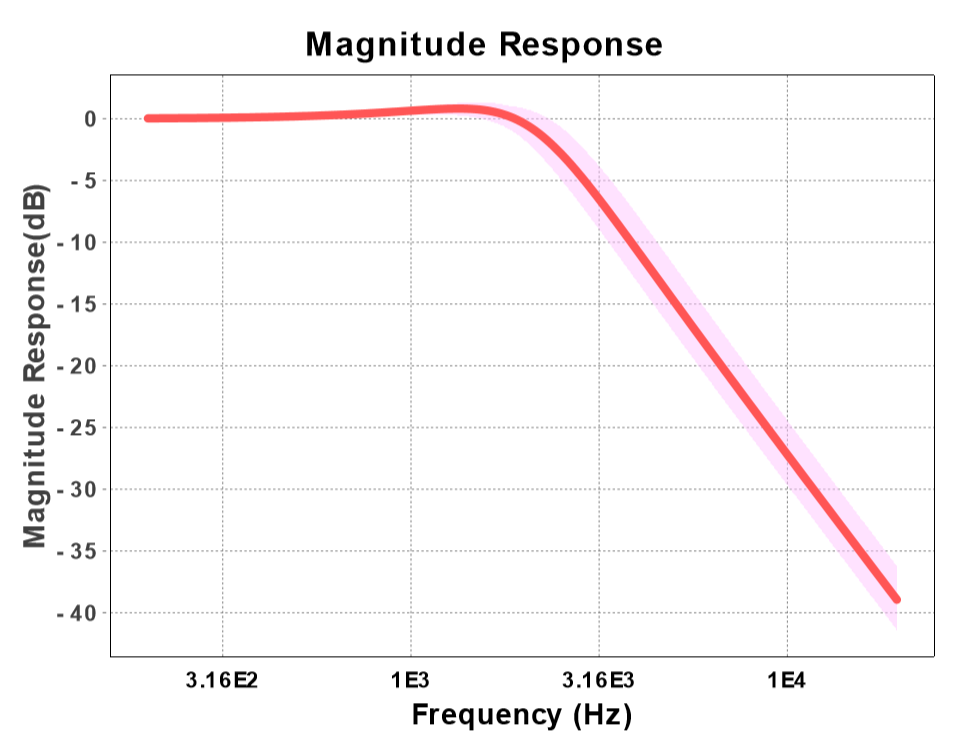
\includegraphics[scale=0.6]{dB_response_FDT.png}
\end{center}
Posteriormente se construye el esquemático del filtro en SPICE para simularlo y observar si su comportamiento coincide con el que muestra el Filter Design Tool. El circuito queda como sigue:
\begin{center}
    \centering
    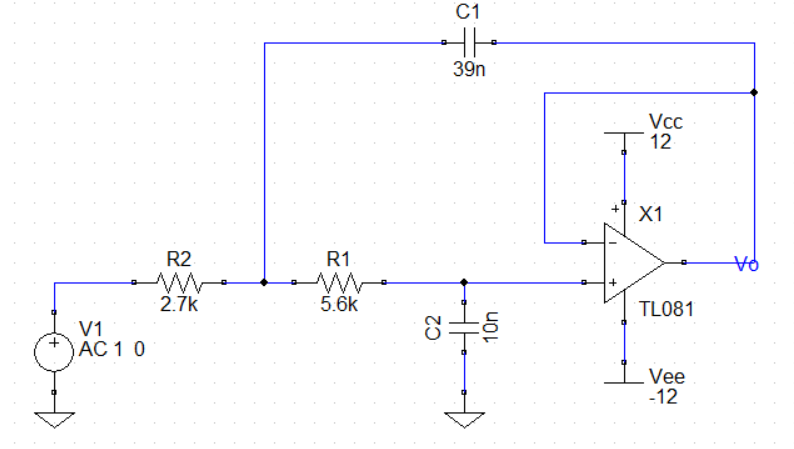
\includegraphics[scale=0.6]{Diagrama_LPF.png}
\end{center}
Se hace una simulación en barrido AC, obteniendo las siguientes gráficas:
\begin{center}
    \centering
    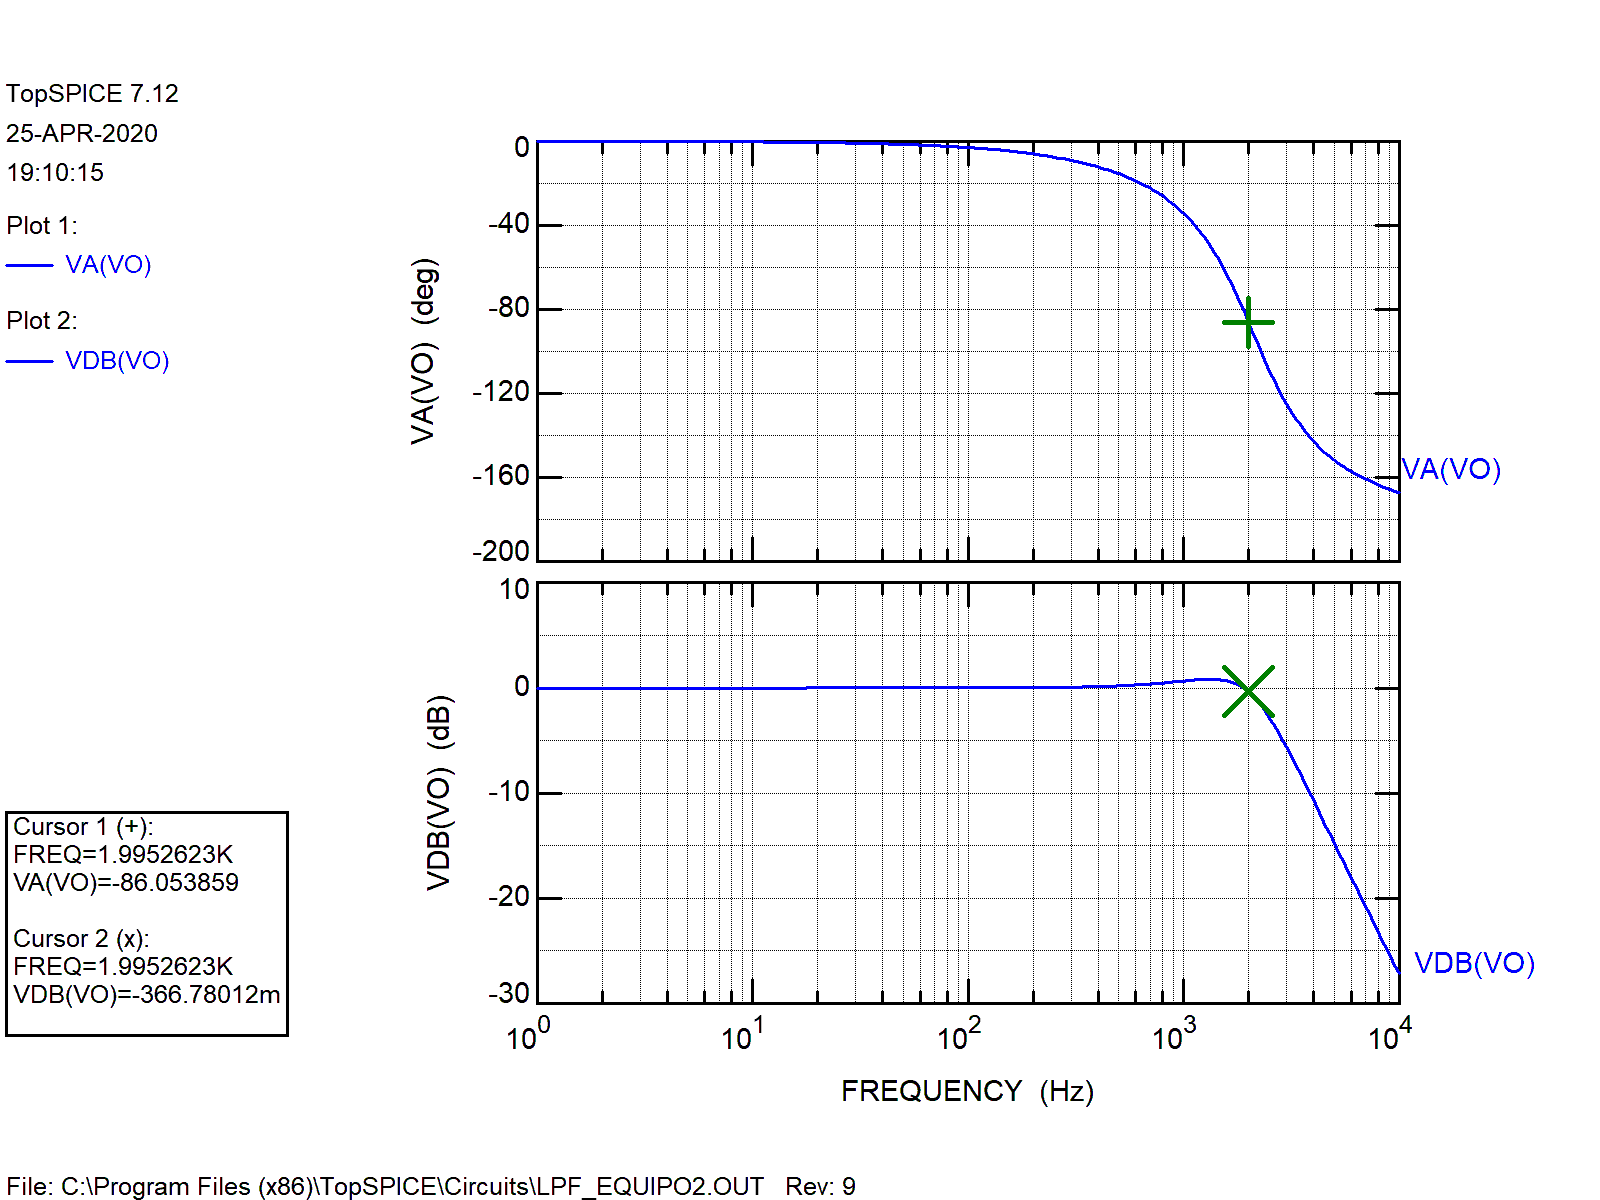
\includegraphics[scale=0.2]{LPF_Equipo2.png}
\end{center}
Como siguiente paso, se hacen variadas simulaciones de análisis en transiente suministrando señales senoidales a diferentes frecuencias, para ser exactos en un rango de 1700-2300 Hz en pasos de 50Hz. Lo anterior para observar como el filtro atenúa la señal de entrada dependiendo de la frecuencia que tiene. Se obtuvieron 13 gráficas diferentes y de los resultados se generó una gráfica que sintetiza los datos obtenidos para hacer más sencillo su análisis.
\begin{center}
    \centering
    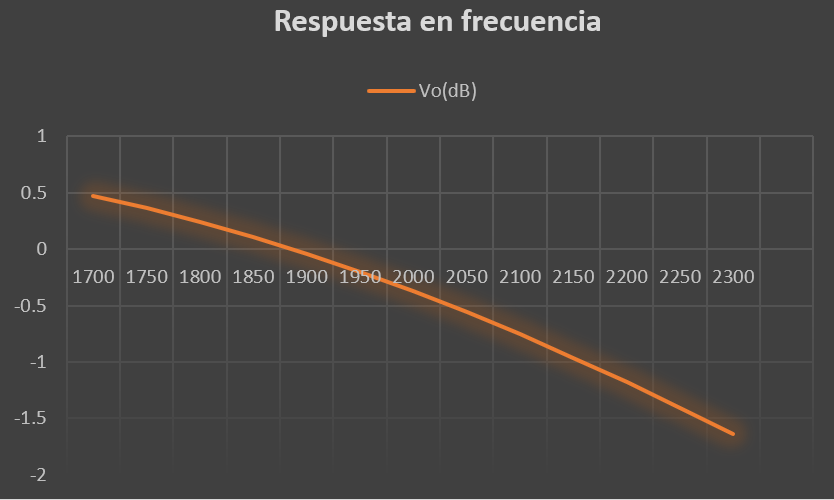
\includegraphics[scale=0.6]{dB_response_calc.png}
\end{center}
\section{Resultados}
Se puede observar en las 3 gráficas diferentes que muestran la respuesta del filtro en el dominio de la frecuencia una similitud bastante notable. Se observa en las primeras dos, la que genera Filter Design Tool y SPICE respectivamente, que hay un pequeño tope o elevación en la rodilla de la gráfica. Esta elevación provoca que en la frecuencia de corte del filtro (2kHz) se tenga una magnitud de aproximadamente -367mdB y no los -3dB que es el parámetro esperado. Este "tope" es una consecuencia de utilizar un filtro Chevyshev, se puede decir que es una desventaja que se compensa con una pendiente en la banda de transición más inclinada a comparación de un Butterworth, lo que significa que el filtro rechazará frecuencias superiores a la de corte de manera más efectiva que el Butterworth. 
\\
Obsérvese además que, en la gráfica que se creó a partir de las simulaciones en el dominio del tiempo, el valor en dB que se obtuvo en 2kHz es de -373mdB. Cifra muy aproximada a la que se obtuvo en SPICE, como consecuencia a esta semejanza se corrobora que este sería el comportamiento del filtro si se llegase a implementar. 
\newpage
\section{Cuestionario}
\textbf{1.Verifique la respuesta en frecuencia del filtro y compare con los resultados obtenidos con Filter Design Tool. ¿Encontró variaciones importantes entre ellas?}
\\
Como ya se mencionó en el apartado de los resultados, las variaciones entre la gráfica de FDT, SPICE y la generada por nosotros son mínimas. Es un comportamiento bastante ideal y es satisfactorio que se haya logrado.
\\
\\
\textbf{2.Compare las gráficas de respuesta en frecuencia obtenidas en los pasos 3 y 4 y realice comentarios.}

A continuacion se muestran los resultados obtenidos en el dominio del tiempo para todo el rango dentro de 1700Hz a 2300Hz.
\begin{figure}[h]
    \centering
    \begin{subfigure}{0.49\textwidth}
    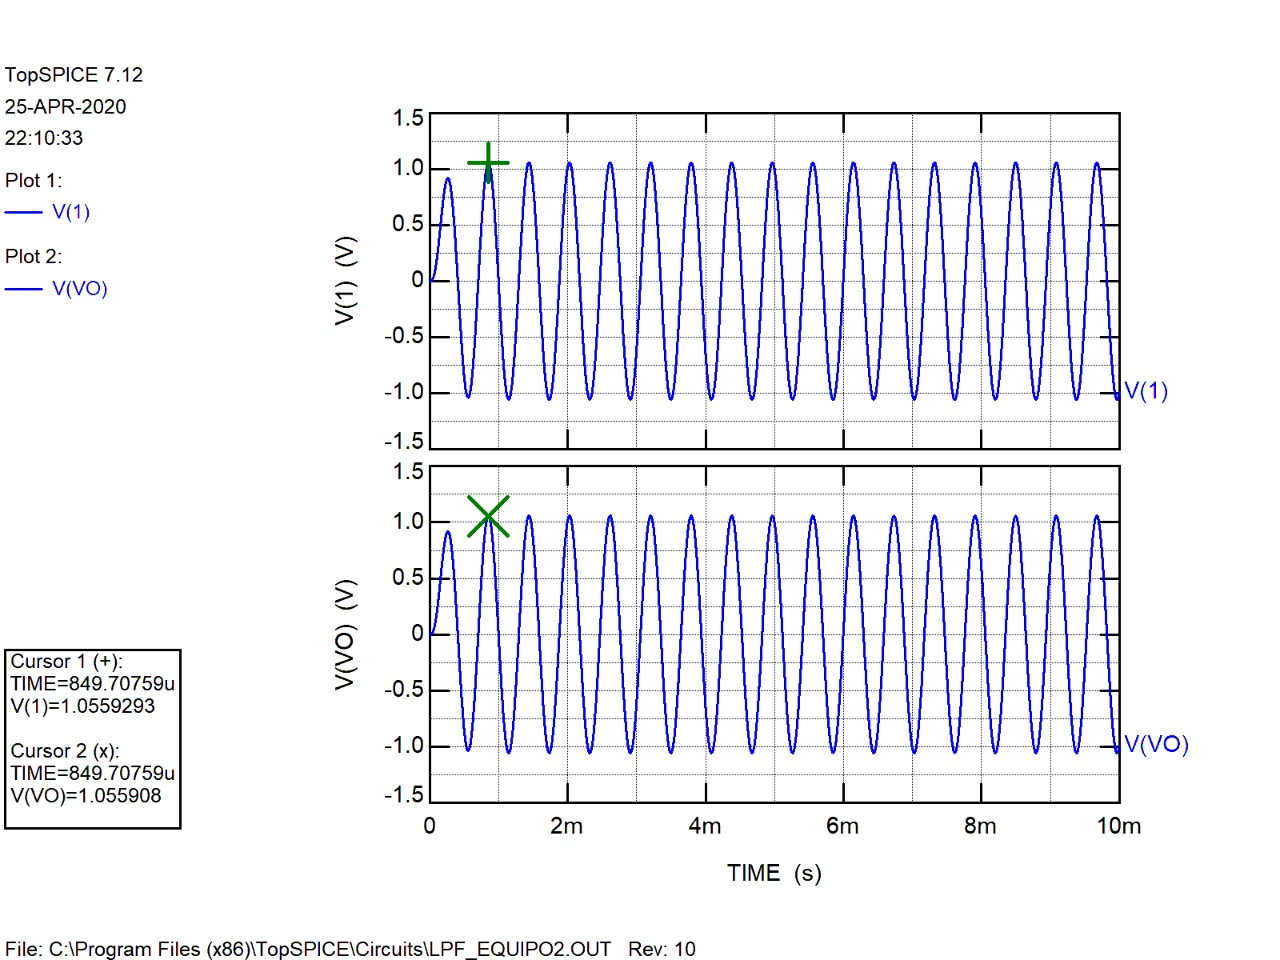
\includegraphics[width=0.9\linewidth]{fig11.jpeg}
    \caption{1700Hz}
    \label{fig:11}
    \end{subfigure}
    \begin{subfigure}{0.49\textwidth}
        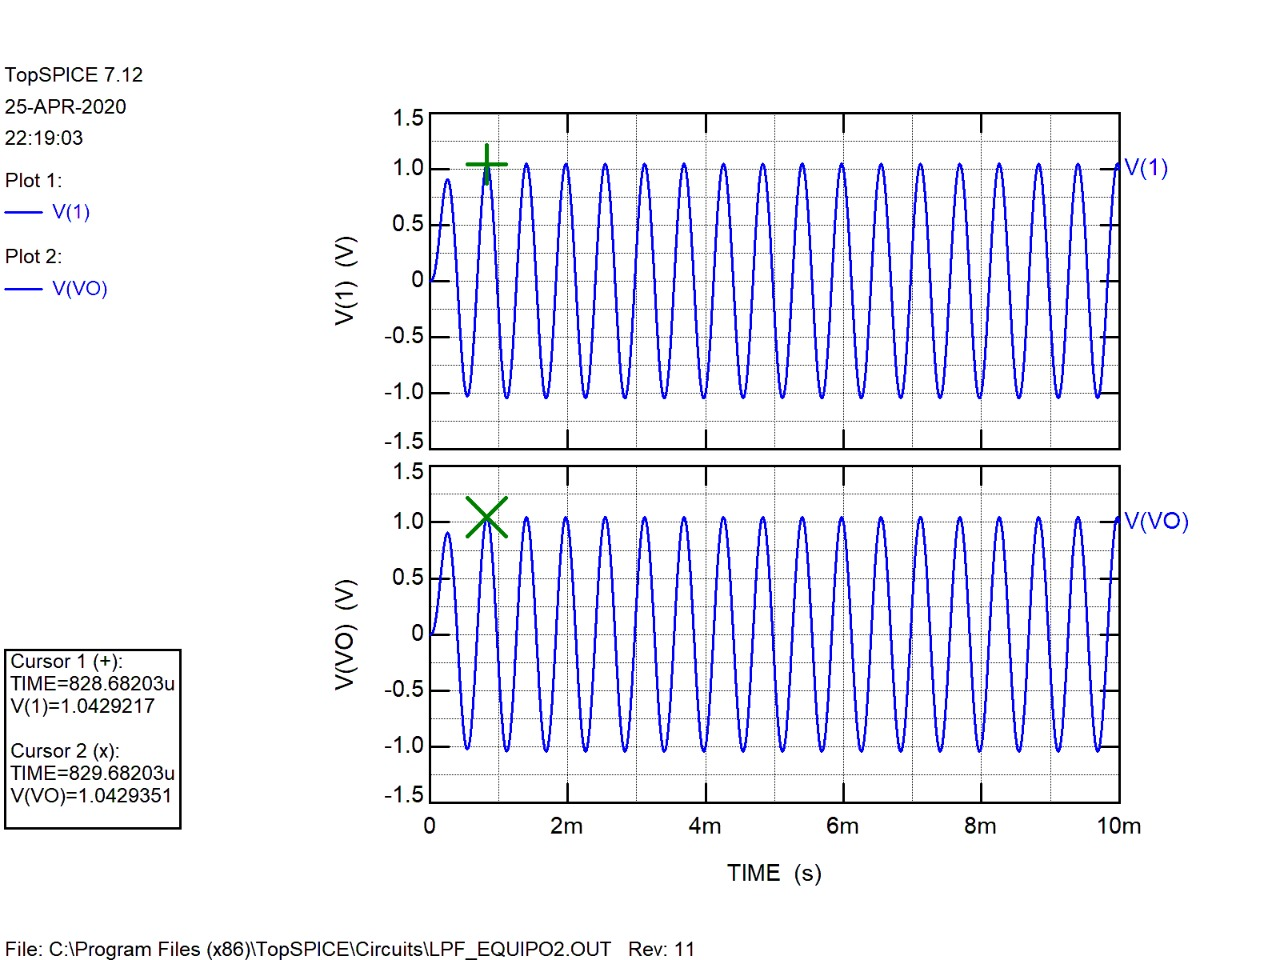
\includegraphics[width=0.9\linewidth]{fig12.jpeg}
        \caption{1750Hz}
        \label{fig:11}
    \end{subfigure}
    \begin{subfigure}{0.49\textwidth}
        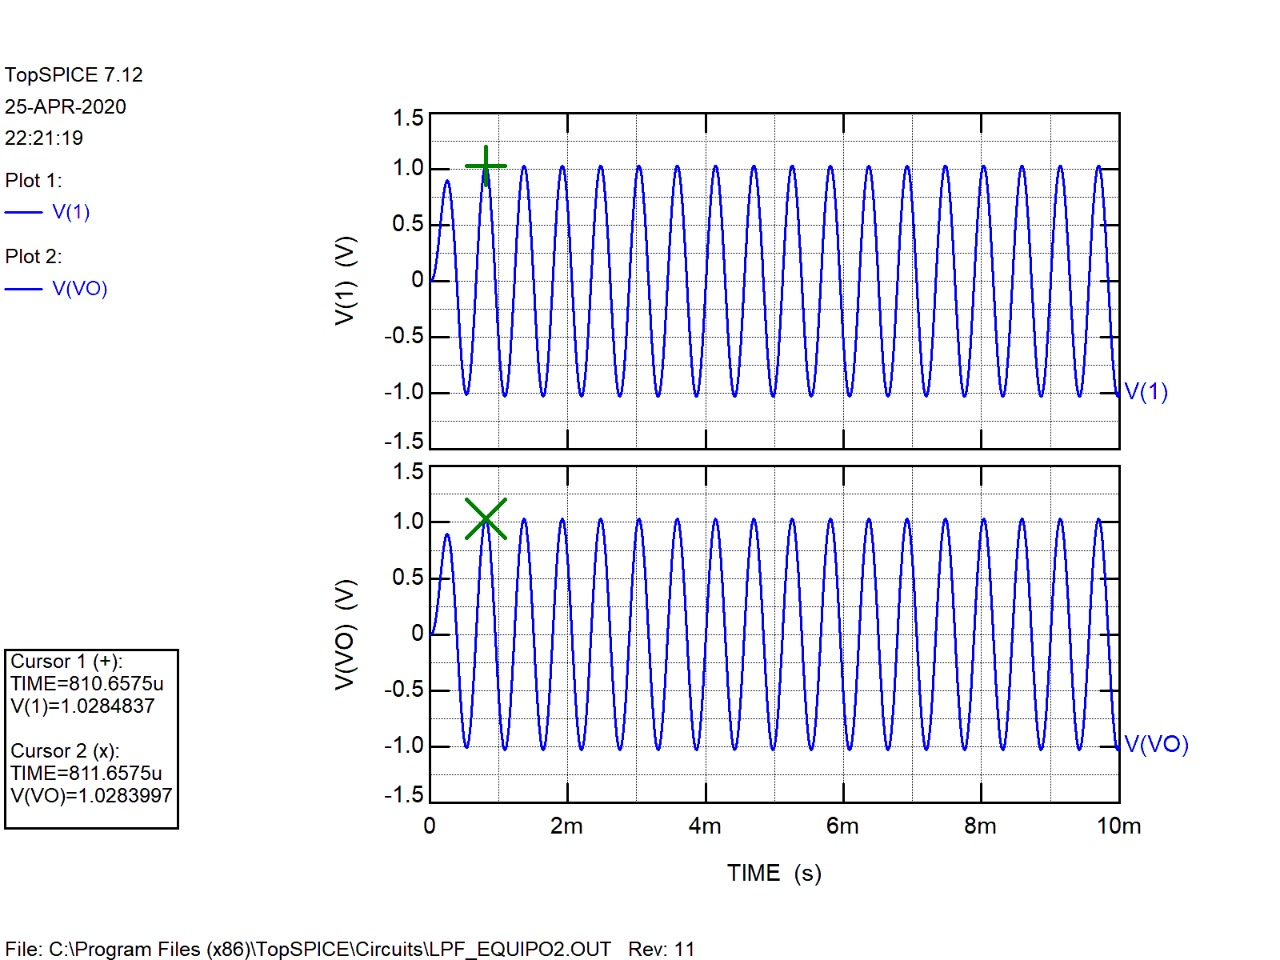
\includegraphics[width=0.9\linewidth]{fig13.jpeg}
        \caption{1700Hz}
        \label{fig:11}
    \end{subfigure}
    \begin{subfigure}{0.49\textwidth}
        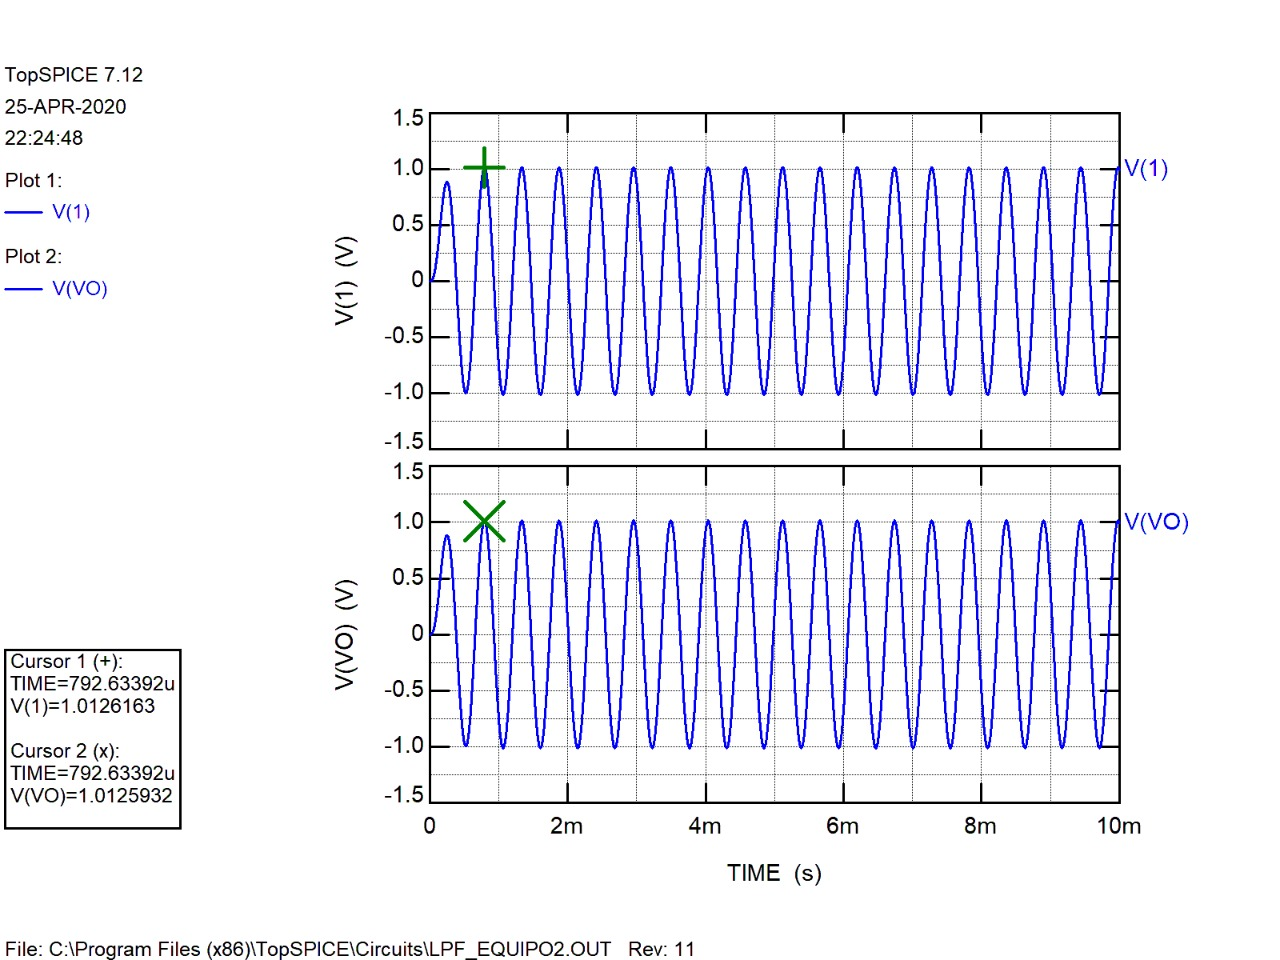
\includegraphics[width=0.9\linewidth]{fig14.jpeg}
        \caption{1800Hz}
        \label{fig:11}
    \end{subfigure}
    \begin{subfigure}{0.49\textwidth}
        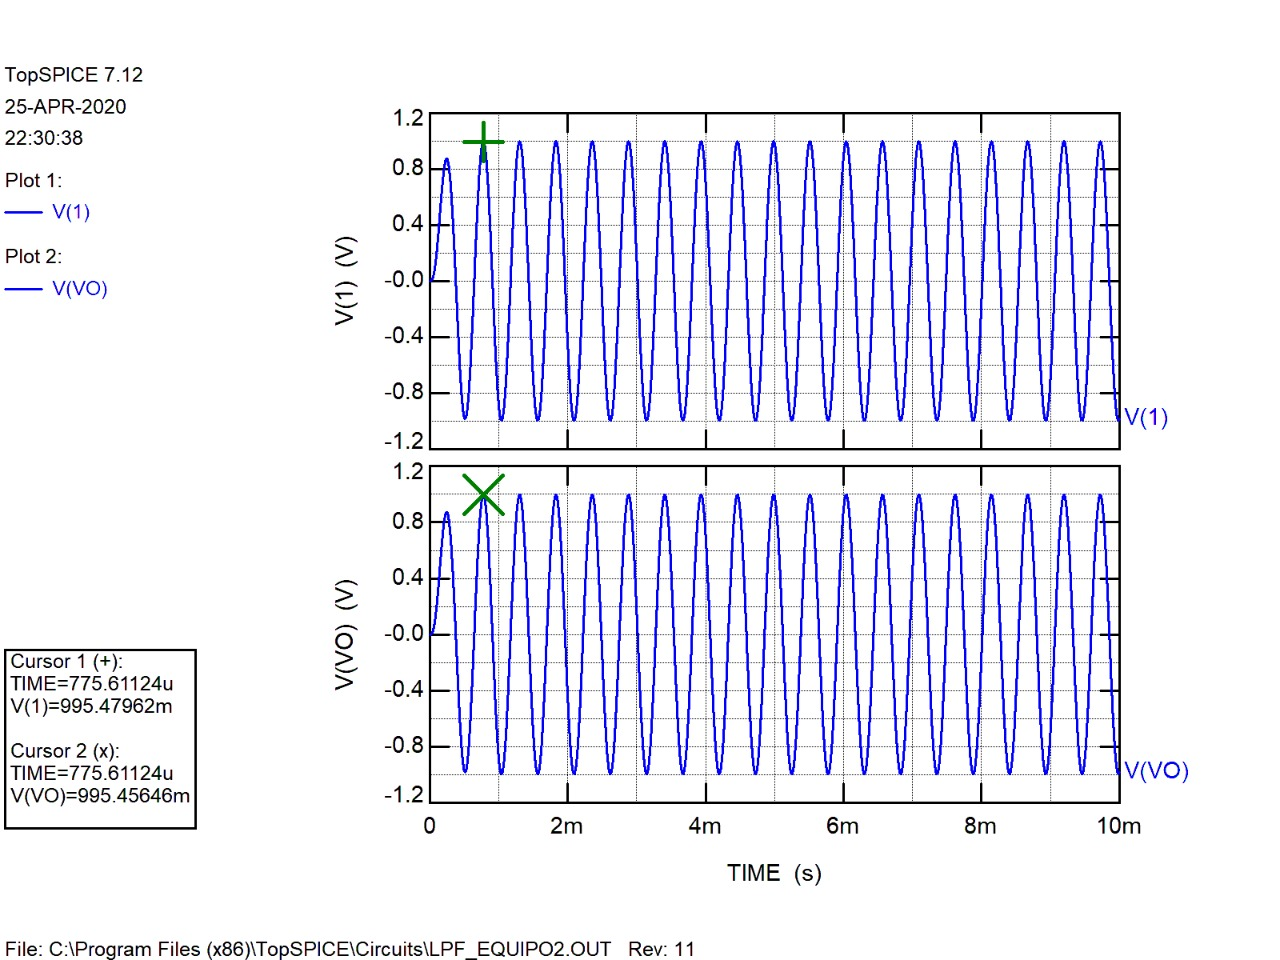
\includegraphics[width=0.9\linewidth]{fig15.jpeg}
        \caption{1850Hz}
        \label{fig:11}
    \end{subfigure}
    \begin{subfigure}{0.49\textwidth}
        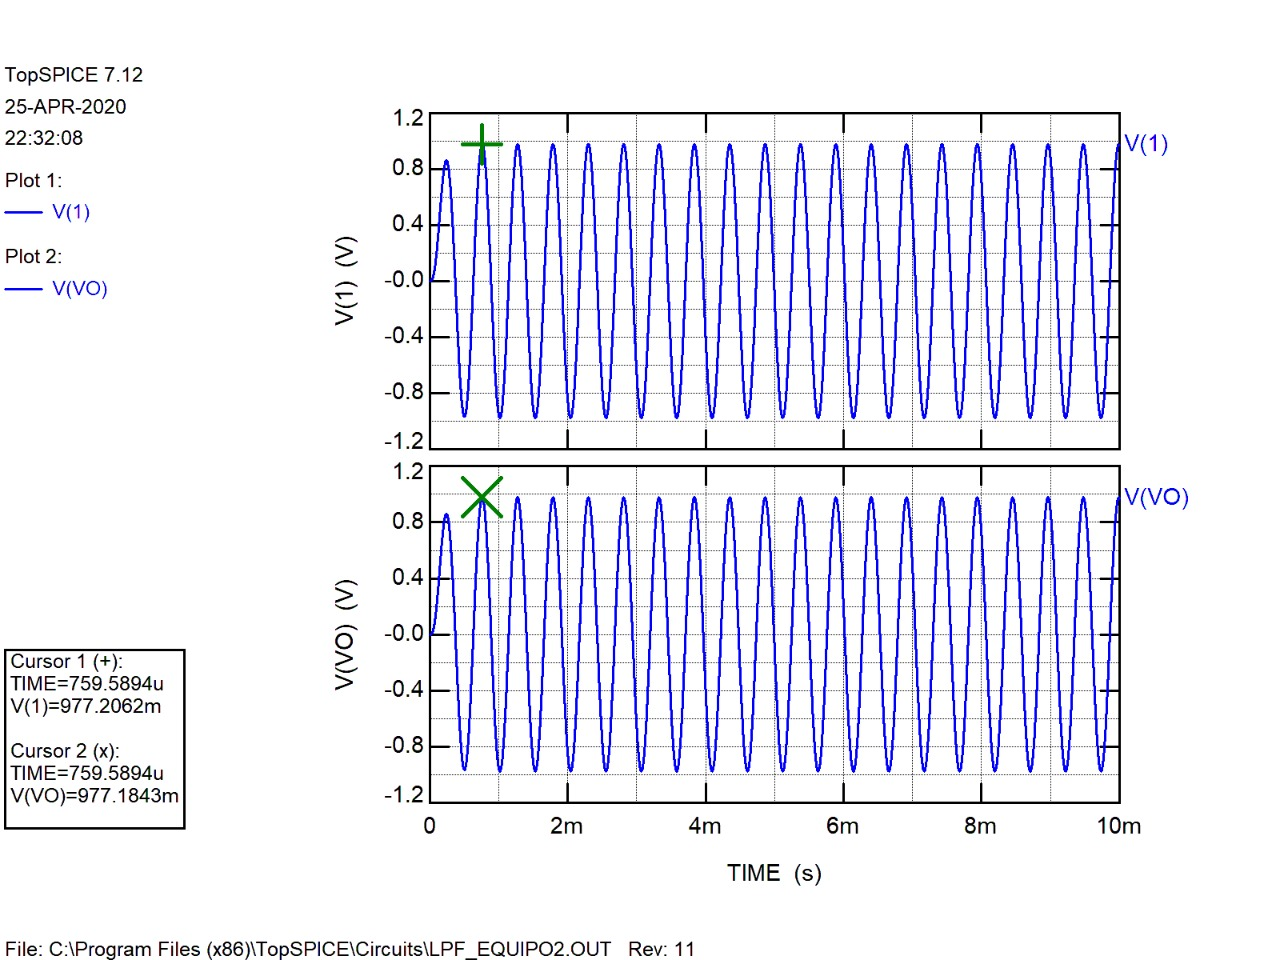
\includegraphics[width=0.9\linewidth]{fig16.jpeg}
        \caption{1900Hz}
        \label{fig:11}
    \end{subfigure}
\end{figure}

\begin{figure}[h]
    \centering
    \begin{subfigure}{0.49\textwidth}
        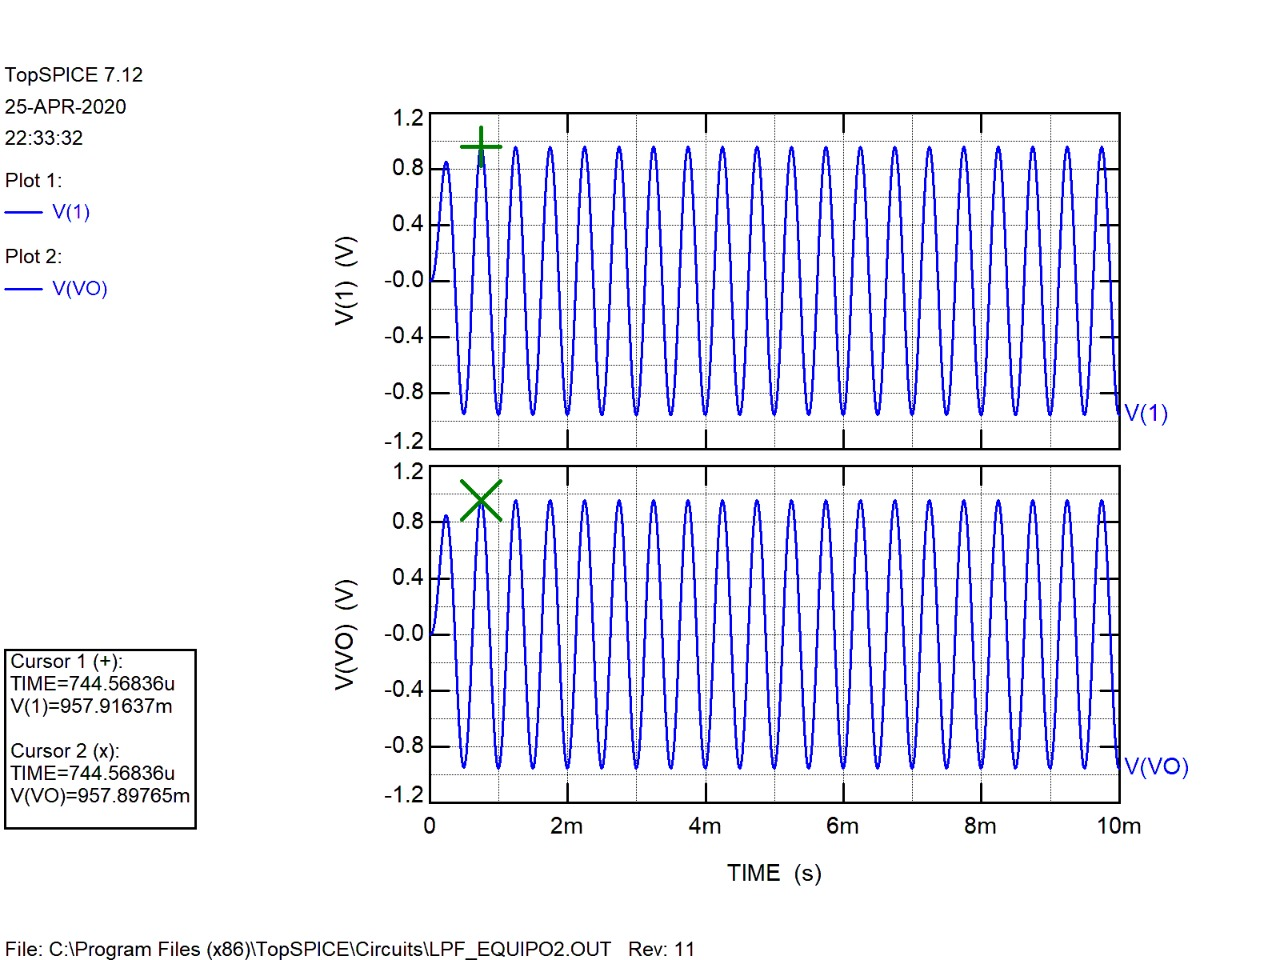
\includegraphics[width=0.9\linewidth]{fig17.jpeg}
        \caption{1950Hz}
        \label{fig:11}
    \end{subfigure}
    \begin{subfigure}{0.49\textwidth}
        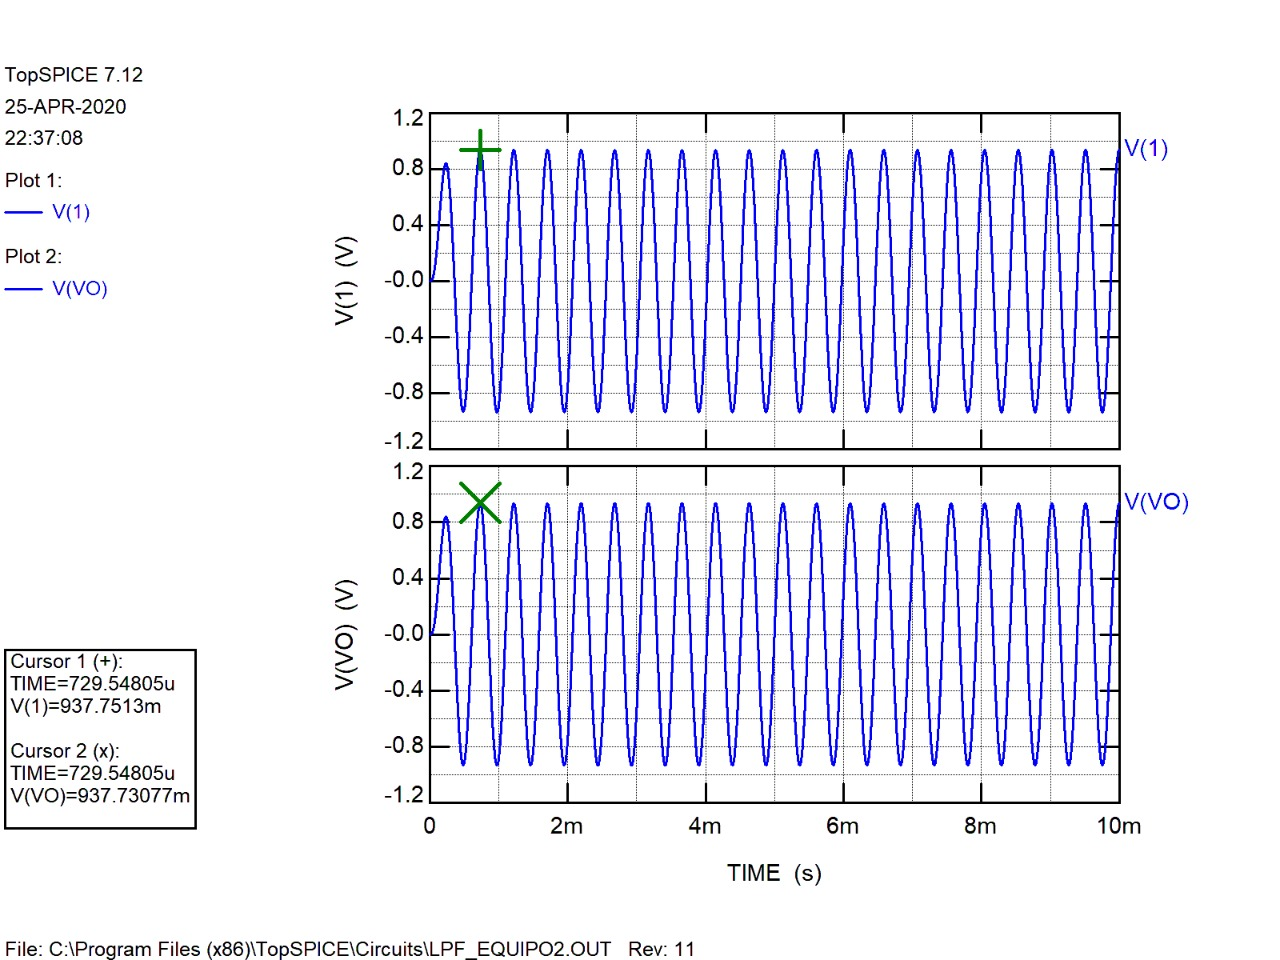
\includegraphics[width=0.9\linewidth]{fig18.jpeg}
        \caption{2000Hz}
        \label{fig:11}
    \end{subfigure}
    \begin{subfigure}{0.49\textwidth}
    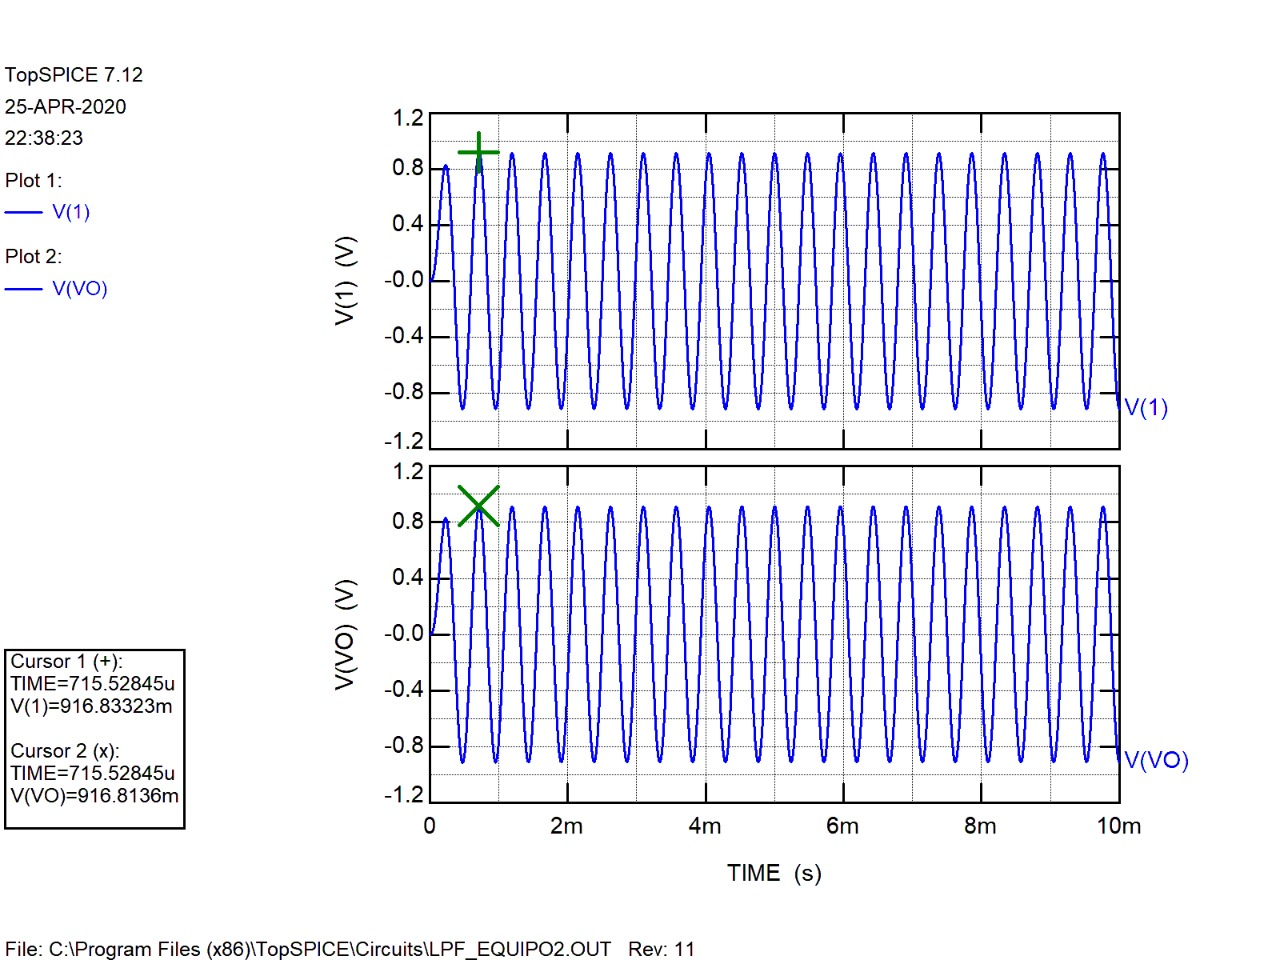
\includegraphics[width=0.9\linewidth]{fig19.jpeg}
    \caption{2050Hz}
    \label{fig:11}
    \end{subfigure}
    \begin{subfigure}{0.49\textwidth}
        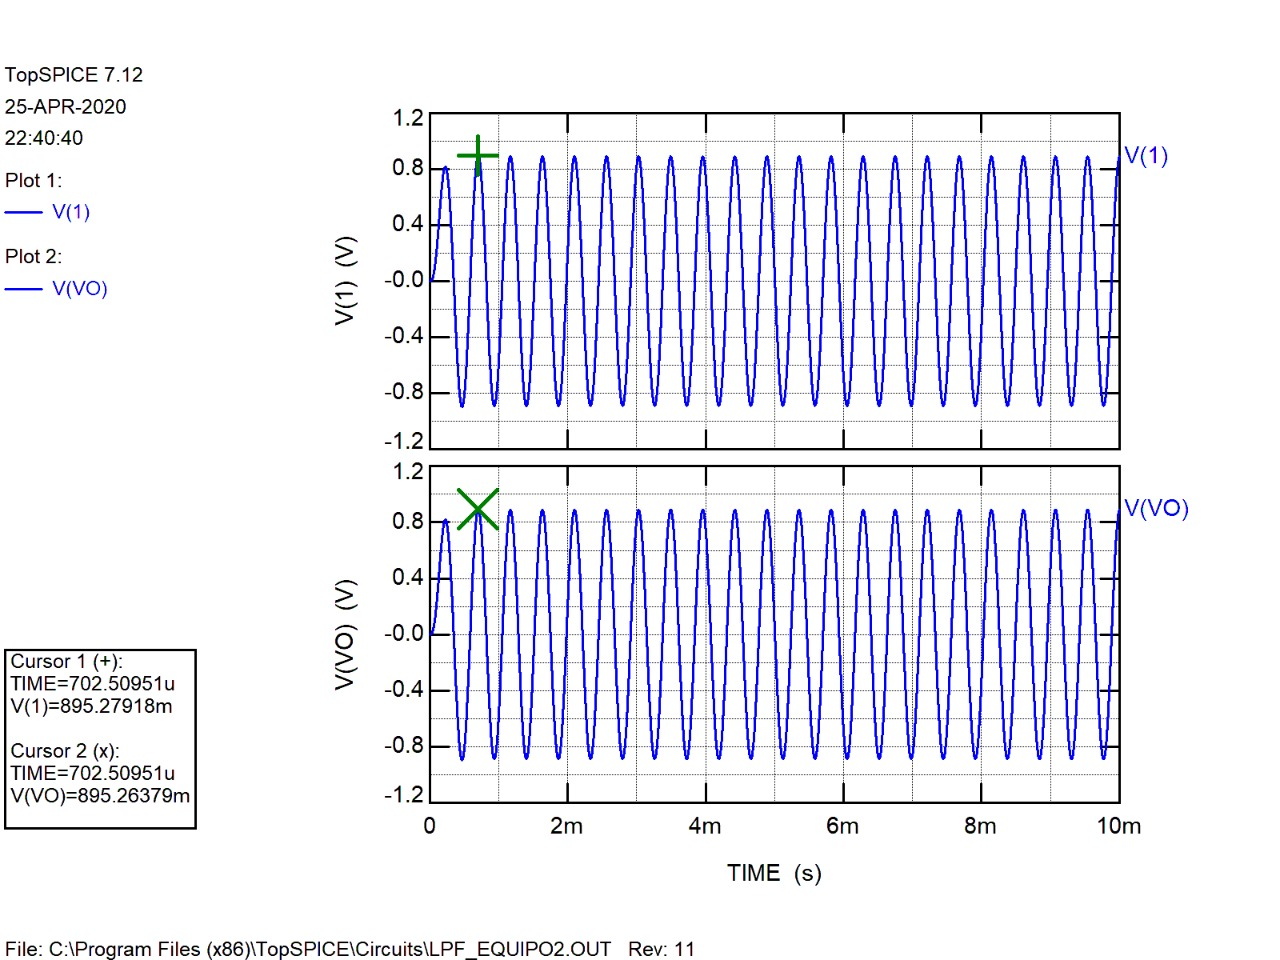
\includegraphics[width=0.9\linewidth]{fig20.jpeg}
        \caption{2100Hz}
        \label{fig:11}
    \end{subfigure}
    \begin{subfigure}{0.49\textwidth}
        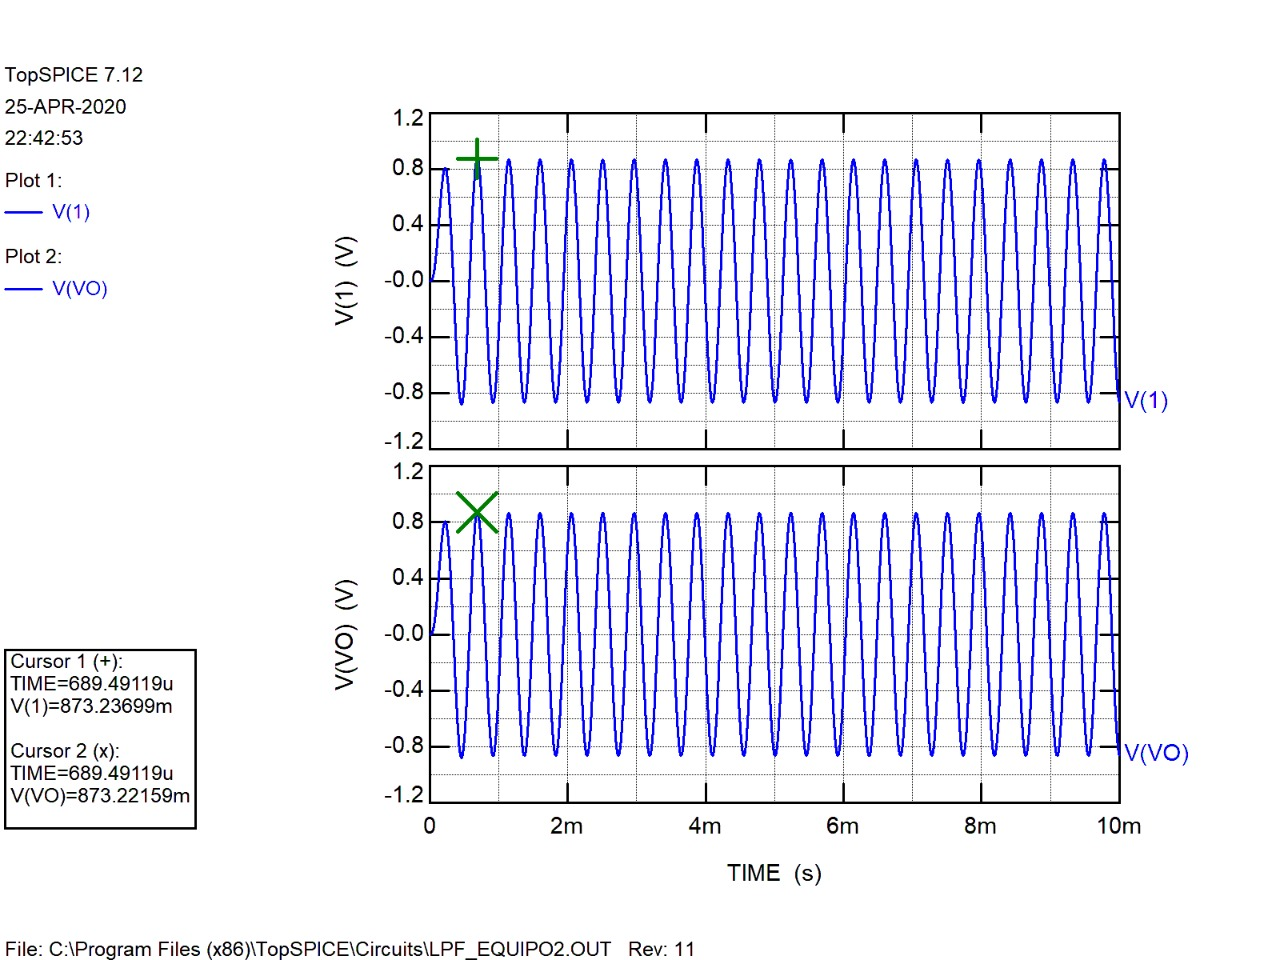
\includegraphics[width=0.9\linewidth]{fig21.jpeg}
        \caption{2150Hz}
        \label{fig:11}
    \end{subfigure}
    \begin{subfigure}{0.49\textwidth}
        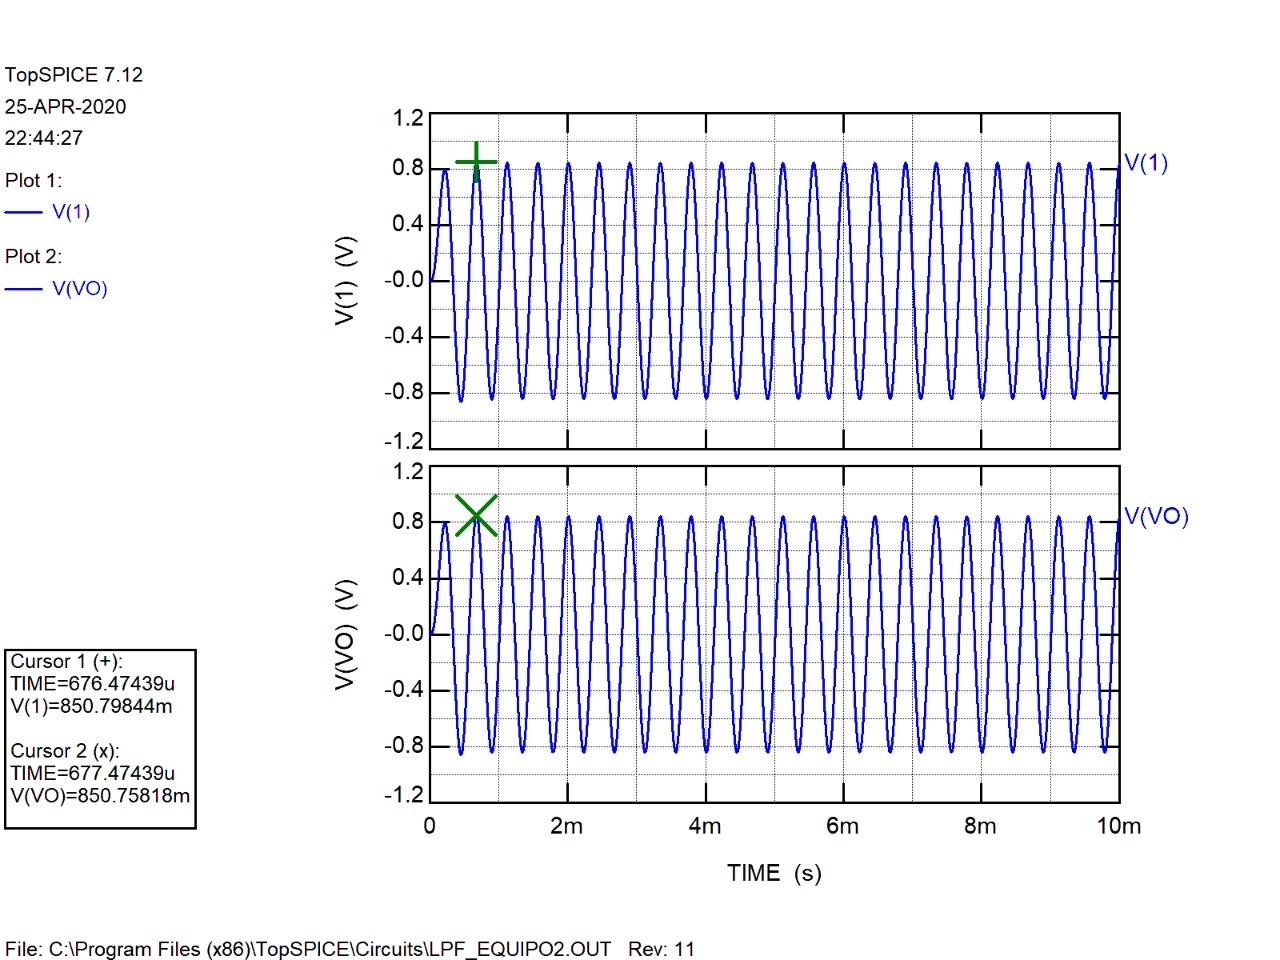
\includegraphics[width=0.9\linewidth]{fig22.jpeg}
        \caption{2200Hz}
        \label{fig:11}
    \end{subfigure}
\end{figure}

\textbf{3. Cuantifique el rizado en banda de paso de su filtro. ¿Se cumplen las características de diseño planteadas  inicialmente?}
\section{Conclusiones}
\bibliographystyle{ieeetr}
\bibliography{biblio}
\section{Apéndice: Códigos.}
\end{document}

